%%
%% 章:生物の特徴
%%------------------------------------------------------------------------------------------------------------------------------%%
\chapter{生物の特徴}
%%
%% 節:いろいろな生物
%%--------------------------------------------------------------------------------------------------------------------%%
\section{いろいろな生物}
%%
%% 項:生物の共通性と多様性
%%----------------------------------------------------------------------------------------------------------%%
\subsection{生物の共通性と多様性}
現在、地球上の約 190 万種類\footnote{未知の生物を含めると数千万種と考えられている。}の(\textcolor{black!10}{種})に名前が付けられている。
\vspc{-0.50zw}\begin{itemize}\setlength{\leftskip}{-1.00zw}%\setlength{\labelsep}{+1.00zw}
\item[\ajMaru{1}](\textcolor{black!10}{種})とは生物の分類の基本的な単位。共通の形態・生理的特徴をもつ集まり。交配で子孫を残すことができる。
\item[\ajMaru{2}] 全ての生物は、共通の祖先から(\textcolor{black!10}{進化})して生じた。進化\footnote{生物の形態が世代を超えて受け継がれ、時間とともに変化していくこと。}は各々の生物が住む生息環境の影響を受けている。
\item[\ajMaru{3}](\textcolor{black!10}{系統樹})とは進化に基づく類縁関係を表す図。系統樹は、従来、生物の形態などを手がかりに作成されてきた。しかし、現在では遺伝情報に基づいた(\textcolor{black!10}{分子系統樹})が作成されている。
\end{itemize}\vspc{-0.50zw}
\vspc{-5.00pt}\begin{figure}[H]\centering\scalebox{1.00}{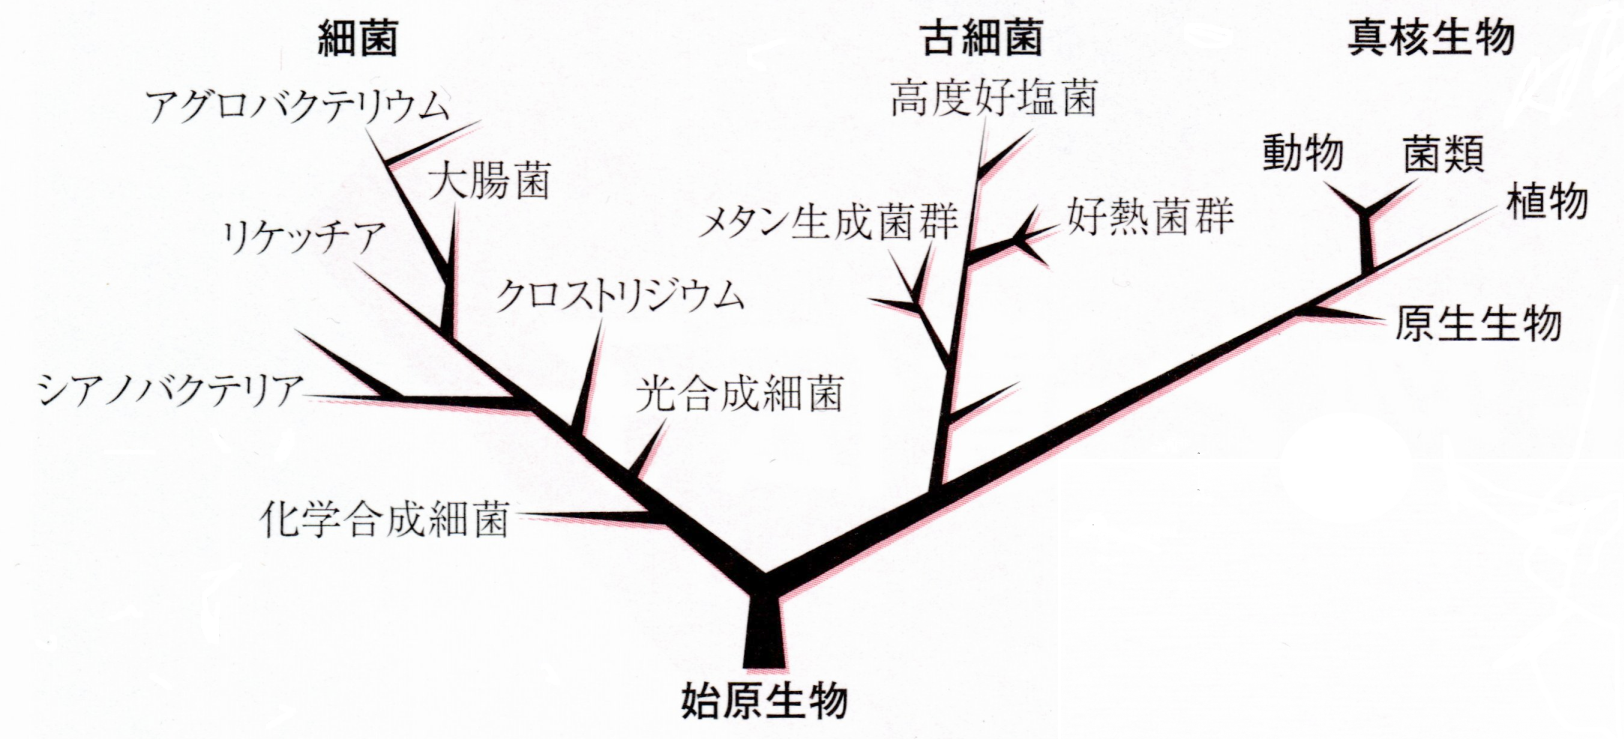
\includegraphics{./Fig/Fig01_01.PNG}}\caption{分子系統樹(大略を示したもの)}\label{分子系統樹}\end{figure}\vspc{-2.00zw}
%%
%% 項:生物の進化
%%----------------------------------------------------------------------------------------------------------%%
\subsection{生物の進化}
\vspc{-0.50zw}\begin{itemize}\setlength{\leftskip}{-1.00zw}%\setlength{\labelsep}{+1.00zw}
\item[\ajMaru{1}] 共通の祖先は約(\textcolor{black!10}{40})億年前に誕生した(\textcolor{black!10}{単})細胞の(\textcolor{black!10}{原核})生物\footnote{細胞内に明確な核がなくDNAが裸の状態で存在している生物。}であったと考えられている。
\item[\ajMaru{2}] 約(\textcolor{black!10}{27})億年前に、\textbf{光合成}によって発生した(\textcolor{black!10}{酸素})が大気中に蓄積し、有害な紫外線を吸収する\textbf{オゾン層}も上空に形成された。これにより生物の陸上進出が可能となった。
\item[\ajMaru{3}] 核膜を持つ(\textcolor{black!10}{真核})生物が誕生する。体が 1 個の細胞からなる(\textcolor{black!10}{単細胞})生物から、多くの細胞からなる(\textcolor{black!10}{多細胞})生物の順に進化した。真核生物の細胞内では呼吸を行う(\textcolor{black!10}{ミトコンドリア})や光合成を行う(\textcolor{black!10}{葉緑体})などの(\textcolor{black!10}{細胞小器官})が生じた。
\end{itemize}\vspc{-1.50zw}
%%
%% 節:生物の共通性
%%--------------------------------------------------------------------------------------------------------------------%%
\section{生物の共通性}
多くの生物に共通する特徴としては\textbf{細胞}・\textbf{代謝}・\textbf{遺伝情報}・\textbf{体内環境の維持}が挙げれる。
%%
%% 項:細胞
%%----------------------------------------------------------------------------------------------------------%%
\subsection{細胞}
全ての生物のからだは(\textcolor{black!10}{細胞})からできている。
\vspc{-0.50zw}\begin{itemize}\setlength{\leftskip}{-1.00zw}%\setlength{\labelsep}{+1.00zw}
\item[\ajMaru{1}](\textcolor{black!10}{単})細胞生物 … からだが\textbf{1 個の細胞}からできている生物。
\item[\ajMaru{2}](\textcolor{black!10}{多})細胞生物 … からだが\textbf{多くの細胞}からできている生物。
\end{itemize}\vspc{-1.50zw}
%%
%% 項:代謝
%%----------------------------------------------------------------------------------------------------------%%
\subsection{代謝}
\vspc{-0.50zw}\begin{itemize}\setlength{\leftskip}{-1.00zw}%\setlength{\labelsep}{+1.00zw}
\item[\ajMaru{1}] 全ての生物は(\textcolor{black!10}{エネルギー})の出入りを伴う(\textcolor{black!10}{代謝})を行う。\enlargethispage{0.50zw}
\item[\ajMaru{2}](\textcolor{black!10}{アデノシン三リン酸:ATP})とはエネルギーの受け渡しを担う物質であり、全ての生物で共通して用いられる。
\end{itemize}\vspc{-1.50zw}
%%
%% 項:遺伝情報
%%----------------------------------------------------------------------------------------------------------%%
\subsection{遺伝情報}
全ての生物は(\textcolor{black!10}{デオキシリボ核酸:DNA})を\textbf{遺伝情報}を記す物質として用いている。
\vspc{-0.50zw}\begin{itemize}\setlength{\leftskip}{-1.00zw}%\setlength{\labelsep}{+1.00zw}
\item[\ajMaru{1}] 生物の形質は DNA の情報を元に作られる(\textcolor{black!10}{タンパク質})により決まる。
\item[\ajMaru{2}](\textcolor{black!10}{生殖})により生物が増殖する際、その種の遺伝情報を持った DNA が子孫に渡される。
\end{itemize}\vspc{-1.50zw}
%%
%% 項:体内環境の維持
%%----------------------------------------------------------------------------------------------------------%%
\subsection{体内環境の維持}
\vspc{-0.50zw}\begin{itemize}\setlength{\leftskip}{-1.00zw}%\setlength{\labelsep}{+1.00zw}
\item[\ajMaru{1}] 全ての生物は、体内の状態を(\textcolor{black!10}{一定})に保つ調節を行っている。
\item[\ajMaru{2}] 体内環境を一定に保つ性質を(\textcolor{black!10}{恒常性:ホメオスタシス})という。
\end{itemize}\vspc{-1.50zw}
%%
%% 節:細胞の特徴
%%--------------------------------------------------------------------------------------------------------------------%%
\section{細胞の特徴}
生物の基本単位を(\textcolor{black!10}{細胞})という。
遺伝子の本体である DNA や様々な物質が(\textcolor{black!10}{細胞膜})によって包まれた構造をもつ。
\vspc{-0.50zw}\begin{itemize}\setlength{\leftskip}{-1.00zw}%\setlength{\labelsep}{+1.00zw}
\item[\ajMaru{1}](\textcolor{black!10}{真核})細胞 … DNA が膜に包まれて\textbf{核}の中に含まれる細胞\footnote{ヒト・ウニなどの動物、ムラサキツユクサ・オオカナダモなどの植物、酵母菌・シイタケなどの菌類、ゾウリムシ・アメーバなどの原生生物。}。
\item[\ajMaru{2}](\textcolor{black!10}{原核})細胞 … DNA が\textbf{細胞内に露出}している細胞\footnote{ネンジュモなどのシアノバクテリア、大腸菌、乳酸菌などの細菌類。}。
\end{itemize}\vspc{-1.50zw}
%%
%% 項:真核細胞の構造
%%----------------------------------------------------------------------------------------------------------%%
\subsection{真核細胞の構造}
(\textcolor{black!10}{核})と(\textcolor{black!10}{細胞質})からなる。
\vspc{-5.00pt}\begin{figure}[H]\centering\scalebox{1.00}{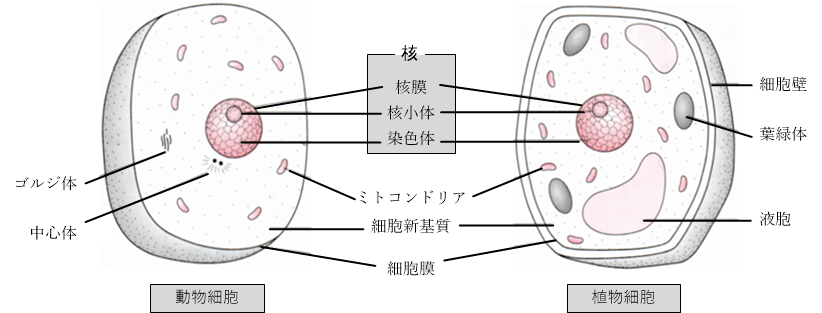
\includegraphics{./Fig/Fig01_02.PNG}}\caption{光学顕微鏡で観察できる細胞の構造}\label{光学顕微鏡で観察できる細胞の構造}\end{figure}\vspc{-1.00zw}
細胞には核・ミトコンドリア・葉緑体など、様々な細胞小器官が存在する。
\vspc{-0.50zw}\begin{itemize}\setlength{\leftskip}{-1.00zw}%\setlength{\labelsep}{+1.00zw}
\item[\ajMaru{1}] \textbf{核} …(\textcolor{black!10}{オルセイン})や(\textcolor{black!10}{カーミン})でよく染まる(\textcolor{black!10}{染色体})が存在する。直径 3 ~ 10\,[$\mu\text{m}$]。(\textcolor{black!10}{核液})に満たされた内部には、1 ~ 数個の(\textcolor{black!10}{核小体})をもつ。(\textcolor{black!10}{核膜})には多数の(\textcolor{black!10}{核膜孔})という物質の通路になる孔がある。
\item[\ajMaru{2}] \textbf{細胞質} … 細胞の核以外の部分。様々な(\textcolor{black!10}{細胞小器官})の間を(\textcolor{black!10}{細胞質基質})が充たしている。
\item[\ajMaru{3}] \textbf{ミトコンドリア} …(\textcolor{black!10}{細胞呼吸})の場。アデノシン三リン酸(ATP)生産に働く。長さ 1 ~ 数\,[$\mu\text{m}$]。
\item[\ajMaru{4}] \textbf{葉緑体} … 植物細胞において、光のエネルギーを用いて有機物を合成する反応である(\textcolor{black!10}{光合成})の場となる。緑色の色素である(\textcolor{black!10}{クロロフィル})を含む。直径 5 ~ 10\,[\ajLig{microm}]。\vspc{-0.50zw}\begin{center}※\textbf{色素体} =\textbf{葉緑体}+(\textcolor{black!10}{白色体})+(\textcolor{black!10}{有色体})\end{center}
\end{itemize}\vspc{-1.50zw}
\vspc{+1.00zw}\begin{figure}[H]\centering\scalebox{1.00}{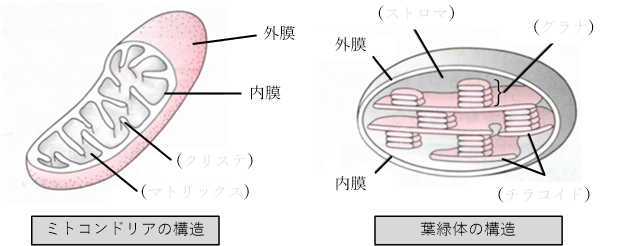
\includegraphics{./Fig/Fig01_03.PNG}}\end{figure}\vspc{-1.00zw}
\vspc{-0.50zw}\begin{itemize}\setlength{\leftskip}{-1.00zw}%\setlength{\labelsep}{+1.00zw}
\item[\ajMaru{5}] \textbf{液胞} … 成熟した植物細胞で特に大きく発達する。内部は(\textcolor{black!10}{細胞液})という液体で満たされ、タンパク質や糖、無機塩類の貯蔵、(\textcolor{black!10}{アントシアン})などの色素を含む。細胞の成長に伴って、細胞の体積に占める割合が大きくなる。水分や物質濃度の調整、老廃物の貯蔵にも関与する。
\item[\ajMaru{6}] \textbf{ゴルジ体} … 物質の(\textcolor{black!10}{分泌})に関わる。分泌\footnote{細胞内から細胞外への物質輸送}の盛んな細胞\footnote{腺細胞など}でよく発生する。
\item[\ajMaru{7}] \textbf{中心体} … 細胞分裂の際に(\textcolor{black!10}{紡錘糸})形成の起点となる。また、ゾウリムシなどがもつ(\textcolor{black!10}{繊毛})の形成に関係する。動物細胞・藻類の細胞やコケ植物・シダ植物の一部の植物細胞に存在する。
\item[\ajMaru{8}] \textbf{細胞質基質} … 液状で様々な酵素などを含み、化学反応の場となる。細胞小器官が流れるように動く(\textcolor{black!10}{原形質流動})が見られる。
\item[\ajMaru{9}] \textbf{細胞膜} … 全ての細胞に存在する厚さ 5 ~ 10\,[\text{nm}] の膜。リン脂質とタンパク質からなる。
  \vspc{-0.00zw}\begin{itemize}\setlength{\leftskip}{-1.00zw}%\setlength{\labelsep}{+1.00zw}
  \item[(1)] \textbf{リン脂質} … 親水性部分と疎水性部分をもち、親水性部分を外に向け二重層構造をとる。
  \item[(2)] \textbf{タンパク質} … リン脂質の二重層構造の中にモザイク状に分布する。物質の輸送や刺激の受容、情報伝達などに関わる。
  \end{itemize}\vspc{-0.00zw}
\item[\ajMaru{10}] \textbf{細胞壁} … 植物細胞や菌類の細胞に存在する。植物細胞の細胞壁は主成分である(\textcolor{black!10}{セルロース})と、細胞の接着に関わる(\textcolor{black!10}{ペクチン})を成分とする。細胞の成長に伴い、特定の物質が沈着(\textcolor{black!10}{リグニン沈着}:木化、(\textcolor{black!10}{スベリン沈着}:コルク化))することがある。
\end{itemize}\vspc{-1.50zw}
%%
%% 項:原核細胞の構造
%%----------------------------------------------------------------------------------------------------------%%
\subsection{原核細胞の構造}
細胞内に(\textcolor{black!10}{核})をもたず、DNA は(\textcolor{black!10}{細胞質})に存在する。
ミトコンドリアや葉緑体などの(\textcolor{black!10}{細胞小器官})をもたないが、細胞膜や(\textcolor{black!10}{細胞壁})はもつ。
運動器官として(\textcolor{black!10}{べん毛})や(\textcolor{black!10}{線毛})をもつものも存在する。
\vspc{-0.50zw}\begin{longtable}{@{}cccc@{}}
  \caption[]{細胞の構造\label{細胞の構造}}                                                                                                                                                                 \\[-1.30zw]\toprule
  \textgt{細胞の構造} & \hspc{+2.00zw}\textgt{原核細胞}\hspc{+2.00zw}                & \textgt{真核細胞(植物)}                                               & \textgt{真核細胞(動物)}                 \\ \midrule\midrule
  核                  &(\textcolor{black!10}{\textbf\textbigcircle})\hspc{+0.00zw} & \hspc{+0.50zw}\textbigcircle{}                                          & \textbigcircle{}                          \\
  細胞壁              &(\textcolor{black!10}{\textbf\textbigcircle})\hspc{+0.00zw} & \hspc{+0.50zw}\textbigcircle{}                                          &(\textcolor{black!10}{\Large\texttimes}) \\
  細胞膜              &(\textcolor{black!10}{\textbf\textbigcircle})\hspc{+0.00zw} &(\textcolor{black!10}{\textbigcircle})                                 &(\textcolor{black!10}{\textbigcircle})   \\
  ミトコンドリア      &(\textcolor{black!10}{\Large\texttimes})                    &(\textcolor{black!10}{\textbigcircle})                                 &(\textcolor{black!10}{\textbigcircle})   \\
  葉緑体              & {\Large\texttimes}                                           & \hspc{+0.50zw}\textbigcircle{}                                          & {\Large\texttimes}                        \\
  発達した液胞        & {\Large\texttimes}                                           & \hspc{+0.50zw}\textbigcircle{}                                          & {\Large\texttimes}                        \\
  ゴルジ体            & {\Large\texttimes}                                           & \hspc{+0.50zw}\hphantom{${}^{\text{※}}$}\textbigcircle${}^{\text{※}}$ & \textbigcircle{}                          \\
  中心体              & {\Large\texttimes}                                           & \hspc{+0.50zw}{\Large\texttimes}                                        & \textbigcircle{}                          \\ \bottomrule
\end{longtable}\vspc{-2.50zw}
\begin{flushright}{\small ※ゴルジ体は植物細胞にも存在するが、植物細胞のゴルジ体は小さく光学顕微鏡で観察することは難しい。}\end{flushright}\vspc{-1.00zw}
%%
%% 節:細胞分画法
%%--------------------------------------------------------------------------------------------------------------------%%
\section{細胞分画法}
細胞小器官を細胞から分離して集める方法を\textbf{細胞分画法}という。
\vspc{-0.50zw}\begin{itemize}\setlength{\leftskip}{-1.00zw}%\setlength{\labelsep}{+1.00zw}
\item[\ajMaru{1}] 手順
  \vspc{-0.50zw}\begin{itemize}\setlength{\leftskip}{-1.00zw}%\setlength{\labelsep}{+1.00zw}
  \item[(1)] 組織をすりつぶして\textbf{細胞破砕液(ホモジェネート)}を作る。この際、細胞内の分解酵素の働きを抑えるために\textbf{低温}で、また細胞小器官の変形を防ぐために\textbf{細胞とほぼ同じ塩類濃度}で行う。
  \end{itemize}\vspc{-0.50zw}

\end{itemize}\vspc{-0.50zw}
